\documentclass[10pt]{article}
\usepackage[utf8]{inputenc}
\usepackage[T1]{fontenc}
\usepackage{amsmath}
\usepackage{amsfonts}
\usepackage{amssymb}
\usepackage[version=4]{mhchem}
\usepackage{stmaryrd}
\usepackage{graphicx}
\usepackage[export]{adjustbox}
\graphicspath{ {./images/} }

\begin{document}
\section*{Math 141 Tutorial 1 Solutions}
\section*{Main problems}
\begin{enumerate}
  \item Compute the following sums and simplify your answer to a single number\\
(a) $\sum_{i=-2}^{2}(2 i+1)$\\
(d) $\sum_{i=2}^{5} \frac{i^{2}-2 i+1}{i-1}$\\
(b) $\sum_{i=-2}^{2} 2 i+1$\\
(e) $\sum_{i=-1}^{1} 2^{i}$\\
(c) $\sum_{i=1}^{4} \frac{1}{i}+1$\\
(f) $\sum_{i=1}^{4} \log _{24} i$
\end{enumerate}

Solutions:\\
(a) $\sum_{i=-2}^{2}(2 i+1)=\sum_{i=1}^{5}(2(i-3)+1)=\sum_{i=1}^{5}(2 i-5)=2 \sum_{i=1}^{5} i-5 \sum_{i=1}^{5} 1=2 \frac{5 \cdot 6}{2}-5 \cdot 5=5$,\\
(b) $\sum_{i=-2}^{2} 2 i+1=\sum_{i=1}^{5}(2(i-3))+1=2 \sum_{i=1}^{5} i-6 \sum_{i=1}^{5} 1+1=2 \frac{5 \cdot 6}{2}-6 \cdot 5+1=1$,\\
(c) $\sum_{i=1}^{4} \frac{1}{i}+1=\frac{1}{1}+\frac{1}{2}+\frac{1}{3}+\frac{1}{4}+1=\frac{24+12+8+6+24}{24}=\frac{74}{24}$,\\
(d) $\sum_{i=2}^{5} \frac{i^{2}-2 i+1}{i-1}=\sum_{i=2}^{5} \frac{(i-1)^{2}}{(i-1)}=\sum_{i=2}^{5}(i-1)=\sum_{i=1}^{4} i=\frac{4 \cdot 5}{2}=10$,\\
(e) $\sum_{i=-1}^{1} 2^{i}=\frac{1}{2}+1+2=\frac{7}{2}$,\\
(f) $\sum_{i=1}^{4} \log _{24} i=\log _{24}(1 \cdot 2 \cdot 3 \cdot 4)=\log _{24} 24=1$.\\
2. Using Riemann sums with $n$ subintervals, approximate the area under the following curves. Draw a picture in order to visualize the rectangles whose areas are being summed.\\
(a) With $n=4$ and either left or right Riemann sums, approximate the area under the curve of $f(x)=2 x-4$ from $x=2$ to $x=4$. What is the true area?\\
(b) With $n=4$ and both left and right Riemann sums, approximate the area under $f(x)=x^{3}$ from $x=0$ to $x=2$. By using both left and right Riemann sums, one obtains upper and lower bounds for the true area. Which method gives a lower bound on the true area? How do you explain this?\\
(c) What do you expect to happen if we repeat the process in part (b) with $n=6$ ? Should we be closer or further from the "true area"?

Solution:\\
(a) For $n=4$, with the left Riemann sum we have

$$
\begin{aligned}
\sum_{i=1}^{n} f\left(x_{i}\right) \Delta x & =\sum_{i=1}^{4} f\left(2+(i-1) \frac{4-2}{4}\right) \frac{4-2}{4}=\frac{1}{2} \sum_{i=1}^{4}\left(2\left(2+\frac{i-1}{2}\right)-4\right) \\
& =\frac{1}{2} \sum_{i=1}^{4}(4+i-1-4)=\frac{1}{2} \sum_{i=1}^{4} i-\frac{1}{2} \sum_{i=1}^{4} 1=\frac{1}{2} \frac{4 \cdot 5}{2}-\frac{1}{2} 4=3
\end{aligned}
$$

and with the right Riemann sum we have\\
$\sum_{i=1}^{n} f\left(x_{i}\right) \Delta x=\sum_{i=1}^{4} f\left(2+i \frac{4-2}{4}\right) \frac{4-2}{4}=\frac{1}{2} \sum_{i=1}\left(2\left(2+\frac{i}{2}\right)-4\right)=\frac{1}{2} \sum_{i=1}^{4} i=\frac{1}{2} \frac{4 \cdot 5}{2}=5$.\\
To compute the true area, notice that the area under $f(x)$ forms a triangle with base length 2 (length of the interval $[2,4]$ ) and height $4(f(4)=2 \cdot 4-4=4)$.\\
(b) For $n=4$, with the left Riemann sum we have

$$
\sum_{i=1}^{4} f\left(x_{i}\right) \Delta x=\sum_{i=1}^{4}\left(0+(i-1) \frac{2-0}{4}\right)^{2} \frac{2-0}{4}=\frac{1}{8} \sum_{i=1}^{4}(i-1)^{2}=\frac{1}{8} \sum_{i=1}^{4} i^{2}-\frac{1}{4} \sum_{i=1}^{4} i+\frac{1}{8} \sum_{i=1}^{4} 1=\frac{7}{4}
$$

And with the right Riemann sum we have

$$
\sum_{i=1}^{4} f\left(x_{i}\right) \Delta x=\frac{1}{8} \sum_{i=1} i^{2}=\frac{15}{4}
$$

The left Riemann sum gives a lower bound on the true area because $f(x)=x^{2}$ is an increasing function.\\
(c) The true area under $f(x)$ from $x=0$ to $x=2$ is $8 / 3$. If we repeat the process in part $(b)$ with $n=6$, we should be closer to the "true area".\\
3. For each function $f(x)$ and interval, write the (left or right) Riemann sum that approximates the area under the curve for any $n \geq 1$.\\
(a) The area under $f(x)=2 x$ between $x=0$ and $x=2$\\
(b) The area between $f(x)=-x+3$, the x -axis and the lines $x=1$ and $x=4$\\
(c) The area under $f(x)=2 x^{2}+1$ between $x=0$ and $x=2$

Solution:\\
(a) We have $a=0$ and $b=2$, so with the left Riemann sum we have

$$
\sum_{i=1}^{n} f\left(x_{i}\right) \Delta x=\frac{2}{n} \sum_{i=1}^{n} 2\left(0+(i-1) \frac{2}{n}\right)=\frac{2}{n} \sum_{i=1}^{n} 2(i-1) \frac{2}{n}
$$

and with the right Riemann sum we have

$$
\sum_{i=1}^{n} f\left(x_{i}\right) \Delta x=\frac{2}{n} \sum_{i=1}^{n} 2\left(0+i \frac{2}{n}\right)=\frac{2}{n} \sum_{i=1} 2 i \frac{2}{n}
$$

(b) We have $a=1$ and $b=4$, so with the left Riemann sum we have

$$
\sum_{i=1}^{n} f\left(x_{i}\right) \Delta x=\frac{3}{n} \sum_{i=1}^{n}\left(-\left(1+(i-1) \frac{3}{n}\right)+3\right)
$$

and with the right Riemann sum we have

$$
\sum_{i=1}^{n} f\left(x_{i}\right) \Delta x=\frac{3}{n} \sum_{i=1}^{n}\left(-\left(1+i \frac{3}{n}\right)+3\right)
$$

(c) We have $a=0$ and $b=2$, so with the left Riemann sum we have

$$
\sum_{i=1}^{n} f\left(x_{i}\right) \Delta x=\frac{2}{n} \sum_{i=1}^{n}\left(2\left(0+(i-1) \frac{2}{n}\right)^{2}+1\right)
$$

And with the right Riemann sum we have

$$
\sum_{i=1}^{n} f\left(x_{i}\right) \Delta x=\frac{2}{n} \sum_{i=1}^{n}\left(2\left(0+i \frac{2}{n}\right)^{2}+1\right)
$$

\begin{enumerate}
  \setcounter{enumi}{3}
  \item We tackle now the inverse process: for each of the following Riemann sums find a function $f(x)$ and values $a$ and $b$ such that the limit expresses the area above/below $f(x)$ between $x=a$ and $x=b$.
\end{enumerate}

Note: There may be several valid answers for each problem.\\
Hint: Every sum appearing in this problem can be realized as a right Riemann sum.\\
(a) $\sum_{i=1}^{n}\left(\frac{3 i}{n}-3\right) \frac{3}{n}$\\
(b) $\sum_{i=1}^{n} \frac{\left(2+\frac{i}{n}\right)^{2}+\left(2+\frac{i}{n}\right)}{n}$\\
(c) $\sum_{i=1}^{n} \exp \left(\frac{6 i}{n}-2\right) \frac{6}{n}$\\
(d) $\sum_{i=1}^{n}\left(\frac{3 i}{2 n}+\frac{1}{2}\right) \tan \left(\frac{3 i}{2 n}-\frac{3}{2}\right) \frac{3}{2 n}$

Solution:\\
(a) One possible answer is $f(x)=x-3$ with $a=0$ and $b=3$.\\
(b) One possible answer is $f(x)=x^{2}+x$ with $a=2$ and $b=3$.\\
(c) One possible answer is $\left.f(x)=e^{( } x-2\right)$ with $a=0$ and $b=6$.\\
(d) One possible answer is $f(x)=\left(x+\frac{1}{2}\right) \tan \left(x-\frac{3}{2}\right)$ with $a=0$ and $b=3 / 2$.

\section*{Challenge problems}
\begin{enumerate}
  \setcounter{enumi}{4}
  \item Using a combination of left and right Riemann sums with $n=4$, find both an upper and lower bound for the area under $f(x)=2 x-x^{2}$ from $x=0$ to $x=2$.
  \item Another method for approximating the area under a curve is known as the Trapezoidal Rule. Here, instead of using rectangles, trapezoids are used. The area of the trapezoid below $f(x)$ and between the nodes $x_{i}$ and $x_{i+1}$ is given by\\
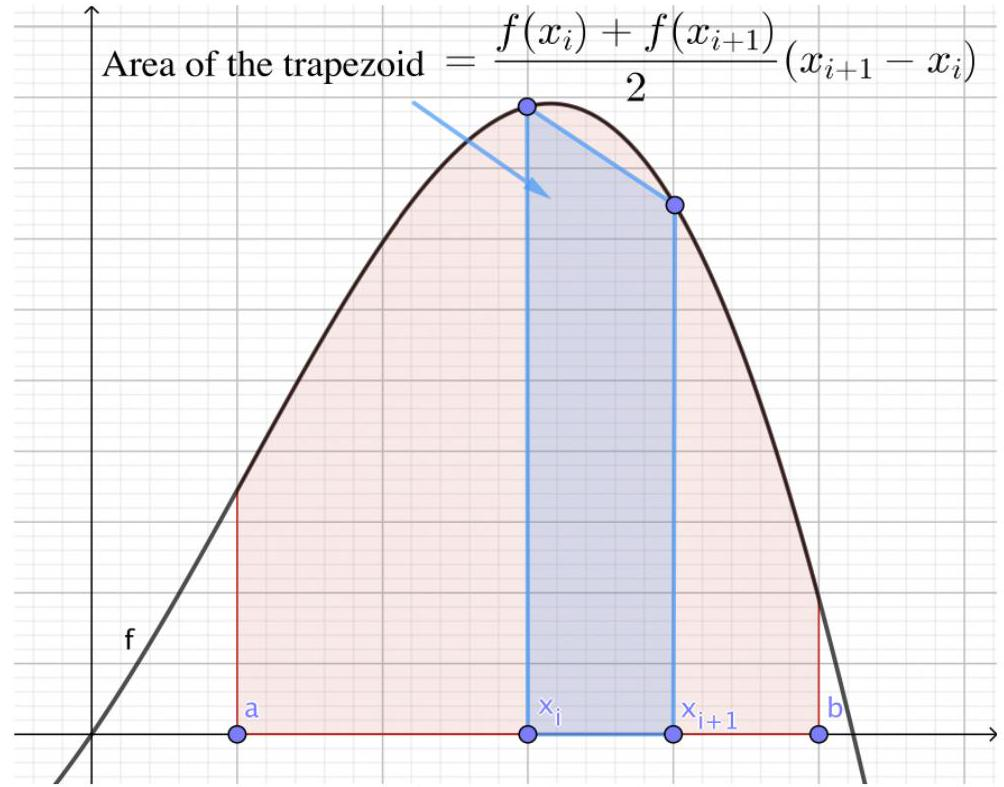
\includegraphics[max width=\textwidth, center]{2024_12_27_54d310dc334f8239f088g-6}\\
(a) Write down an equation for the Trapezoidal Rule when using a fixed number $n$ of trapezoids to approximate the area under $f(x)$ between $x=a$ and $x=b$.\\
(b) Can you write down the formula for the Trapezoidal Rule in terms of left and right Riemann sums?\\
(c) Suppose that both left and right Riemann sums are finite and equal. Can you find the limit of your sum from (b) as $n$ tends to infinity? Does this new approximation still converge to the true area under $f(x)$, between $x=a$ and $x=b$ ?
\end{enumerate}

\end{document}